\documentclass[12pt,a4paper,oneside,titlepage,liststotoc,bibtotoc]{scrreprt}
\usepackage[utf8]{inputenc}
\usepackage[top=2.5cm,bottom=2.5cm,left=2.5cm,right=2.5cm,includehead,includefoot,headsep=1cm]{geometry}
\usepackage[ngerman]{babel}
\usepackage{graphicx}
\usepackage{hyperref}
\usepackage{setspace}
\usepackage{fancyhdr}
\usepackage{acronym}
\usepackage{listings}
\usepackage{float}
\usepackage{enumitem}
\usepackage{listings}
\usepackage{color}
\usepackage{microtype}
\usepackage[toc, nogroupskip, nonumberlist, nopostdot]{glossaries}
\usepackage{array}

% Infos
\newcommand{\titel}{Dokumentation Projektarbeit}
\newcommand{\untertitel}{Bombenspiel}
\newcommand{\arbeit}{}
\newcommand{\pruefung}{Bachelor of Science}
\newcommand{\studiengang}{Informatik}
\newcommand{\studienrichtung}{Angewandte Informatik}
\newcommand{\autor}{Jonas Kümmerlin, Simon Knab, Sandra Kramlich, Marco Herglotz}
\newcommand{\matrikelnr}{}
\newcommand{\kurs}{TINF15B4}
\newcommand{\firma}{}
\newcommand{\abgabe}{22. Juni 2017}
\newcommand{\betreuerdhbw}{}
\newcommand{\betreuerfirma}{}
\newcommand{\jahr}{2017}
\newcommand{\code}[1]{\texttt{#1}}
\newcommand{\source}[1]{\footnotesize Quelle: \url{#1}}
\newcommand{\zitat}[1]{\glqq{}#1\grqq{}}

% Logos
\newcommand{\logodhbw}{
\includegraphics[width=6cm]{img/logos/dhbw}}
\newcommand{\logofirma}{
\includegraphics[width=6cm]{img/logos/dhbw}}

% Definition der Kopf- und Fußzeilen
\fancyhf{}
\fancyhead[L]{\sffamily \autor}
\fancyhead[R]{\sffamily \nouppercase{\leftmark}}
\fancyfoot[C]{\sffamily \thepage}
%\renewcommand{\chapterpagestyle}{scrheadings}

\pagestyle{fancy}
\onehalfspacing

%code style for listings
\definecolor{javared}{rgb}{0.6,0,0} % for strings
\definecolor{javagreen}{rgb}{0.25,0.5,0.35} % comments
\definecolor{javapurple}{rgb}{0.5,0,0.35} % keywords
\definecolor{javadocblue}{rgb}{0.25,0.35,0.75} % javadoc

\renewcommand{\lstlistingname}{Programmcode}
\lstset{language=[x86masm]Assembler,
	basicstyle=\ttfamily\footnotesize,
	keywordstyle=\color{javapurple}\bfseries,
	stringstyle=\color{javared},
	commentstyle=\color{javagreen},
	morecomment=[s][\color{javadocblue}]{/**}{*/},
	tabsize=4,
	showspaces=false,
	showstringspaces=false,
	frame=single,
	breaklines=true,
	captionpos=b
}

\setlist[2]{noitemsep}

\begin{document}

\begin{titlepage}
\sffamily

% Logos
\logodhbw \hfill \\[2ex]

\begin{center}

% Text
\huge{\textsc{\textbf{\titel}}}\\
\Large{\textbf{\untertitel}}\\[4ex]

%\LARGE{\textbf{\arbeit}}\\[4ex]

\normalsize{Für die Prüfung zum\\
\pruefung}\\[4ex]

\Large{Studiengang \studiengang}\\
\normalsize{Studienrichtung \studienrichtung}\\
\normalsize{Duale Hochschule Baden-Württemberg Karlsruhe}\\[4ex]

Von\\
\autor \\[8ex]

% Tabelle
\begin{tabular}{ll}
Abgabedatum:				   	& \quad \abgabe\\
%Matrikelnummer: 			    & \quad \matrikelnr\\ 
Kurs:                           & \quad \kurs\\ 
%Ausbildungsfirma:	 			& \quad \firma\\ 
%Betreuer der Ausbildungsfirma:  & \quad \betreuerfirma
\end{tabular}
    
\end{center}

\end{titlepage}
\chapter*{Eidesstattliche Erklärung}

Erklärung gemäß~§~5~(3) der "`Studien- und Prüfungsordnung DHBW Technik"' vom 29.~September~2015. Wir versichern hiermit, dass wir diese Arbeit selbstständig verfasst und keine anderen als die angegebenen Quellen als Hilfsmittel benutzt haben.\\[4ex]

\noindent Karlsruhe, den \today \\[8ex]
\noindent \rule{5cm}{0.5pt} \\
\noindent \autor\\

\section*{Sperrvermerk}

Der Inhalt dieser Arbeit darf weder als Ganzes noch in Auszügen Personen außerhalb des Prüfungsprozesses und des Evaluationsverfahrens zugänglich gemacht werden, sofern keine anders lautende Genehmigung der Ausbildungsstätte vorliegt.

\section*{Copyright-Vermerk}

Dieses Werk einschließlich seiner Teile ist \textbf{urheberrechtlich geschützt}. Jede Verwertung außerhalb der engen Grenzen des Urheberrechtsgesetzes ist ohne Zustimmung des Autors unzulässig und strafbar. Das gilt insbesondere für Vervielfältigungen, Übersetzungen, Mikroverfilmungen sowie die Einspeicherung und Verarbeitung in elektronischen Systemen.

\begin{flushright}
    \copyright{} \jahr
\end{flushright}

\clearpage

\tableofcontents
\clearpage

\chapter{Einleitung}

\section{Motivation}

Die Motivation der Arbeit war das Vertiefen der vermittelten, theoretischen Inhalte. Erwartet wurde kein umfangreiches Projekt, sondern nur ein kleines, auf einem 8051 Mikrocomputer lauffähiges Programm, welches ein wenig über den vermittelten Lernstoff hinaus reicht und damit das Wissen um Assembler weiter festigt und vertieft.

\section{Aufgabenstellung}

Die Aufgabe war es mit dem erworbenen Wissen aus der Vorlesung \zitat{Systemnahe Programmierung} ein kleines Programm zu entwickeln. Dieses soll dann auf einem 8051 Mikrocomputer mit simulierter Hardware laufen. Die Simulation selbst wird von der verwendeten Entwicklungsumgebung MCU-8051 IDE bereitgestellt. Der 8051 und die IDE werden in Kapitel \ref{section:8051} und \ref{section:ide} genauer vorgestellt.

Wir als Gruppe haben uns das Ziel gesetzt, das bekannte \zitat{Bombenspiel} zu entwickeln. Hierbei wird eine Bombe mit zufälliger Zündschnur zwischen zwei Spielern hin und her geworfen. Der Spieler, bei dem die Bombe explodiert, hat verloren. Das genaue Konzept zu unserer Idee ist in Kapitel \ref{section:konzept} ausführlich erklärt.
\chapter{Grundlagen}

\section{Assembler}

Assembler ist eine Programmiersprache der zweiten Generation und ist ein direkter Nachfolger der Programmierung in Maschinensprache, also mit Zahlencodes. Bei Assembler handelt es sich um eine hardwarenahe Programmiersprache. Je nachdem welche Hardware verwendet wird, stehen unterschiedliche Befehlssätze zur Verfügung. Daher gibt es nicht die \zitat{eine} Programmiersprache Assembler, sondern es handelt sich um eine Gruppe von Assemblersprachen, die für die jeweilige Hardware angepasst ist.\cite{bib:assembler}

Generell handelt es sich bei Assembler um eine zeilenorientierte Sprachfamilie, das heißt eine Zeile stellt immer eine komplette Anweisung dar. Diese Anweisungen bestehen aus den hardware-spezifischen Befehlen.\cite{bib:assembler_book}

\section{Der 8051 Mikrocomputer} \label{section:8051}

Der 8051 Mikrocomputer wurde 1981 von Intel als 8-bit Mikrocontroller auf den Markt gebracht. Es handelt sich um ein \zitat{system on a chip}, was bedeutet, dass RAM, ROM, zwei Timer, ein Serial Port, 4 8-bit Ports und noch einiges mehr auf einem einzigen Chip verbaut sind. Die einzelnen Bestandteile sind in Abbildung \ref{img:8051} dargestellt.\cite{bib:8051} 

Mittlerweile ist der Original 8051 veraltet, dennoch existieren viele Abwandlungen (Derivate) beziehungsweise Weiterentwicklungen des 8051. Diese sind allerdings mit höherer Taktfrequenz und geringerer Taktteilung ausgestattet, sodass sie nahezu auf dem aktuellen Stand der Technik und damit deutlich leistungsfähiger als das Ursprungsmodell sind.\cite{bib:8051_2}

\begin{figure}[htbp]
	\centering
	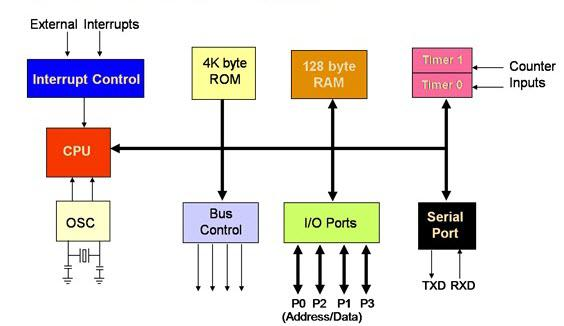
\includegraphics[scale=0.75]{img/8051-diagram}
	\caption{Blockdiagramm eines 8051 Mikrocomputers}
	\label{img:8051}
	\source{https://www.tutorialspoint.com/embedded_systems/images/block_diagram.jpg}
\end{figure}


\section{Entwicklungsumgebung MCU-8051 IDE} \label{section:ide}

Die MCU-8051 IDE ist eine integrierte Entwicklungsumgebung für Mikrocontroller und basiert auf dem 8051 Mikroprozessor. Neben Assembler können die Programme auch in C entwickelt werden.

Die IDE unterstützt den Entwicklungsprozess neben einem Quellcode Editor auch mit einem Simulator zum direkten Ausführen des Programms auf verschiedenen Mikrocontrollern. Auch eine Hardware-Anbindung in Form eines LCD Displays, eines Keypads und vielen weiteren Tools wird von der MCU-8051 IDE bereitgestellt.\cite{bib:mcu}
\chapter{Konzept} \label{section:konzept}

\section{Analyse}

Anfangs soll auf dem Display eine Willkommensnachricht und die bisherige Spielstatistik angezeigt werden. Der Spielablauf beginnt dann mit dem Drücken des Knopfs (im folgenden als Buzzer bezeichnet). In diesem Moment wird die Bombe einem zufälligen Spieler gegeben, der sie dann durch Drücken des Buzzers dem anderen Spieler zuwerfen kann. Nach einer zufälligen Zeit explodiert die Bombe und der Spieler, der sie aktuell hat, verliert diese Runde. Danach wechselt das Spiel zurück in den Startbildschirm und die Statistik wird entsprechend angepasst.

Um obigen Programmablauf realisieren zu können, werden die folgenden Komponenten benötigt:

\begin{itemize}
	\item Timer, für die \zitat{Länge} der Zündschnur
	\item Zufallsgenerator, für die \zitat{Länge} der Zündschnur
	\item LCD Display, zur Darstellung des aktuellen Spielzustandes
	\item Keypad, genauer gesagt ein einziger Knopf zur Steuerung des Spielverlaufs
\end{itemize}

\section{Programmentwurf}

Zur technischen Umsetzung ist der Programmablauf in Abbildung \ref{img:flussdiagramm} geplant.

\begin{figure}[htbp]
	\centering
	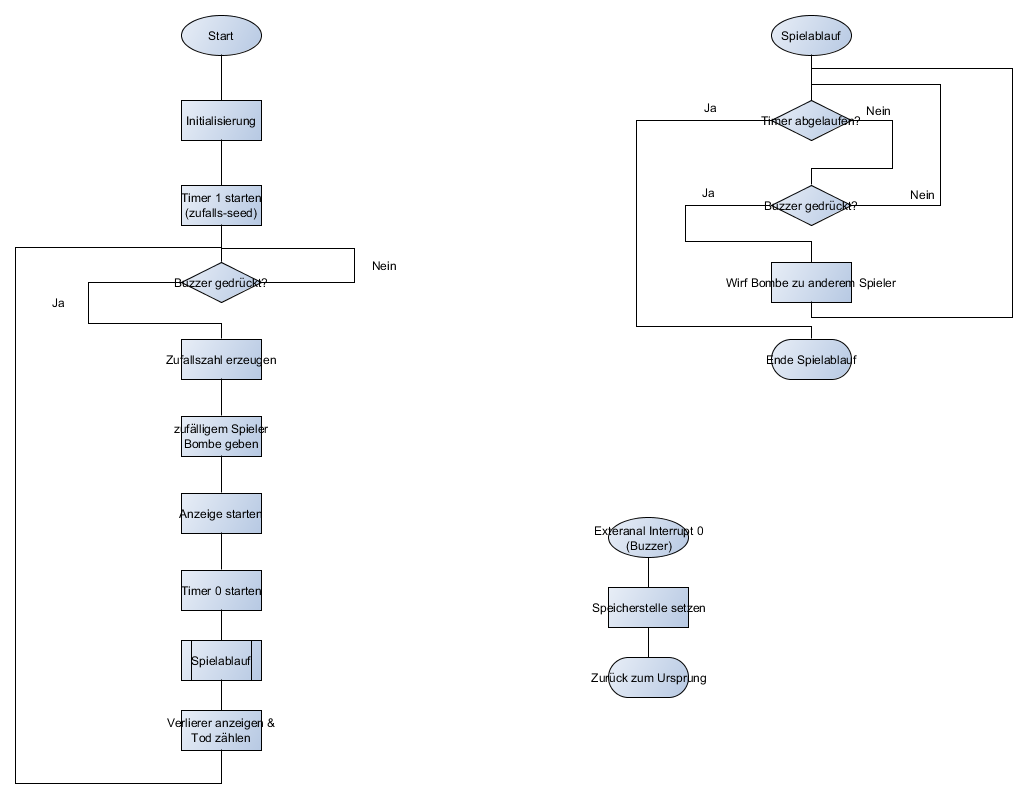
\includegraphics[scale=0.45]{img/Flussdiagramm}
	\caption{Flussdiagramm des Programms}
	\label{img:flussdiagramm}
\end{figure}

Zur Steuerung des Buzzers muss eine Interrupt Routine verwendet werden, um direkt beim Drücken des Buzzers eine Speicherstelle zu setzen. Würde der Buzzer nicht mit einem Interrupt realisiert, könnte es passieren, dass der Spieler den Buzzer bereits wieder losgelassen hat, bevor das Programm an der entsprechenden Verzweigung angekommen ist.


\chapter{Implementierung}

\begin{figure}[htbp]
	\centering
	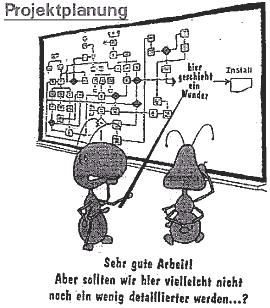
\includegraphics[scale=1.5]{img/wunder}
\end{figure}
\source{http://www.informatik.uni-oldenburg.de/~sos/kurse09/img/projekte.jpg}


\section{Buzzer}

Der Buzzer wurde wie bereits erwähnt mit einer Interrupt Steuerung implementiert. Der Quellcode ist in Programmcode \ref{code:buzzer} abgebildet. 

\noindent
\begin{minipage}[t]{\textwidth}
	\vspace{1em}
	\begin{lstlisting}[caption=Quellcode für den Buzzer Interrupt, label=code:buzzer]
	BUZZER_IR equ p3.2
	BUZZER equ B.0
	
	IRS_init:
	setb EA			;enable Interrupts
	setb EX0		;enable INT0
	setb IT0		;make INT0 edge triggered
	ret
	
	int0_handler:
	setb BUZZER		;set BUZZER
	clr IE0
	reti	
	\end{lstlisting}
\end{minipage}

\section{Zufallsgenerator}

Die Funktion \code{random\_init} wird beim Starten des Programms aufgerufen um den Zufallsgenerator zu initialisieren. Für die erste erzeugte Zufallszahl wird der Wert von \code{Timer1} verwendet und mit der Funktion \code{random\_seed\_from\_timer} in die passende Variable geladen. Danach wird immer \code{random\_next} verwendet, um eine auf der letzten Zufallszahl basierte neue Zufallszahl zu erhalten.

\noindent
\begin{minipage}[t]{\textwidth}
	\vspace{1em}
	\begin{lstlisting}[caption=Quellcode für die Zufallszahlen-Generierung, label=code:random]
; Writes random number in RANDOM_NUM,
; uses last one as seed.
; 8-bit galois lsfr implemented according to wikipedia
random_next:
mov A, RANDOM_NUM

clr C
rrc A ; rotate right
jnc random_skipmask

xrl A,#10111000b		; apply xor mask for x^8+x^6+x^5+x^4+1
random_skipmask:
mov RANDOM_NUM,A

ret

random_init:
mov RANDOM_NUM,#42

; setup timer 1 for random seed values
orl TMOD,#00100000b
anl TMOD,#11101111b
setb TR1

ret

random_seed_from_timer:
mov A,TL1
jnz random_seed_from_timer_nonzero		; our LSFR won't work if all bits are zero
mov A,#0FFh
random_seed_from_timer_nonzero:
mov RANDOM_NUM,A
ret
	\end{lstlisting}
\end{minipage}

\section{Timer}

Der Timer musste deutlich komplizierter realisiert werden als gedacht. Das Spiel soll eine gewissen Zeit laufen, allerdings lassen die Timer des 8051 nur eine sehr geringe Zeitspanne zu, sodass wir dieses Problem umgehen mussten. Ein Ausschnitt des Timer-Codes ist in Programmcode \ref{code:timer} zu sehen. 

\noindent
\begin{minipage}[th]{\textwidth}
	\vspace{1em}
	\begin{lstlisting}[caption=Quellcode-Ausschnitt für die Timerverwaltung, label=code:timer]
	timer_init:					; Subroutine to setup the timer
	mov TL0,TIMER_RELOAD_VAL;	; reset timer counter
	mov TH0,TIMER_RELOAD_VAL+1;
	
	anl TMOD,#11111101b	; intialize timer mode: timer 0 in 16 bit mode
	orl TMOD,#00000001b
	setb TR0;
	setb EA;					; enable timer interrupt
	setb ET0;
	ret;
	
	timer_int_handler:			; timer interrupt handler
	mov R7, A 			; save current acc
	clr IE0			; prevent INT0 from getting triggered with timer ir
	
	mov TL0,TIMER_RELOAD_VAL;
	mov TH0,TIMER_RELOAD_VAL+1;
	mov A,TIMER_DEC_COUNTER
	jz timer_lo_zero
	dec TIMER_DEC_COUNTER
	jmp timer_hi_zero
	timer_lo_zero:
	mov A,TIMER_DEC_COUNTER+1
	jz timer_hi_zero
	dec TIMER_DEC_COUNTER+1
	mov TIMER_DEC_COUNTER,#0FFh
	timer_hi_zero:
	inc TIMER_INC_COUNTER
	
	mov A, R7			; reset acc to state before interrupt
	reti
	\end{lstlisting}
\end{minipage}

\section{LCD Display}

Das LCD Display ist einer der komplizierteren Komponenten aus dem Gesamtprogramm. Die beiden Macros zum Schreiben eines Strings auf das LCD Display sind in Programmcode \ref{code:lcd} dargestellt. Die Komponente selbst ist allerdings deutlich größer, um auch Routinen für das Schreiben der aktuellen Statistik einfach anzubieten.

\noindent
\begin{minipage}[th]{\textwidth}
	\vspace{1em}
	\begin{lstlisting}[caption=Quellcode-Ausschnitt für das LCD Display, label=code:lcd]
lcd_sendChar macro char	;call this macro like   LCD_sendChar #'A'
mov   	LCD_data, char 	;Move the char to LCD port
setb	LCD_rs			;Selected data register
clr	LCD_rw				;We are writing
setb	LCD_en			;Enable H-> L
clr	LCD_en
inc	CURSOR_POS			;save new cursor position
call	LCD_busy		;Wait for LCD to process the data
endm

lcd_sendString macro string
local START				;define local macro label
local EXIT				;define local macro label
mov   dpl, #low(string)
mov   dph, #high(string)
start:					;local labels have to be in lowercase, idk why^^
clr   a                 ;clear Accumulator for any previous data
movc  a,@a+dptr         ;load the first character in accumulator
jz    EXIT              ;go to exit if zero
LCD_sendChar A			;send actual char
inc   dptr              ;increment data pointer
sjmp  START    			;jump back to send the next character
exit:					;local labels have to be in lowercase, idk
endm

	\end{lstlisting}
\end{minipage}

\clearpage
\section{Hauptroutine}

Die Hauptroutine initialisiert zuerst sämtliche Komponenten. \code{gamestart} schreibt dann den \code{BEGIN} Text auf das Display und wartet auf das Drücken des Buzzers. Sobald dieser gedrückt wird, wird die Bombe einem zufälligen Spieler gegeben und danach der Timer auf einen zufälligen Wert gesetzt.In Programmcode \ref{code:main} ist dieser Ablauf zu sehen.

Programmcode \ref{code:loop} zeigt die Hauptschleife in der das Programm läuft. Dabei wird zuerst überprüft, ob der Counter abgelaufen, das heißt die Bombe bereits explodiert ist. Falls nicht, wird der Buzzer überprüft und die \code{toggleActivePlayer} Routine aufgerufen, sofern dieser gedrückt ist. Im Anschluss wird mit \code{sendActivePlayerNumber} das LCD Display aktualisiert.

\noindent
\begin{minipage}[th]{\textwidth}
	\vspace{1em}
	\begin{lstlisting}[caption=Quellcode-Ausschnitt: Hauptschleife, label=code:loop]
	throwBomb:
	; exit game on timeout
	mov A,TIMER_DEC_COUNTER
	orl A,TIMER_DEC_COUNTER+1
	jz game_timeout

	; check for button press
	mov A,BUZZER
	cjne A, #1, throwBomb ; not pressed

	; pressed
	clr BUZZER

	call toggleActivePlayer
	call sendActivePlayerNumber
	ljmp throwBomb
	\end{lstlisting}
\end{minipage}

\noindent
\begin{minipage}[th]{\textwidth}
	\vspace{1em}
	\begin{lstlisting}[caption=Quellcode-Ausschnitt für die Hauptroutine, label=code:main]
	gamestart:
	LCD_setCursor #01h, #00h
	LCD_sendString BEGIN
	
	call waitForBuzzer
	
	; set active player based on random number
	call random_seed_from_timer
	call random_next
	mov A,RANDOM_NUM
	
	mov ACTIVE_PLAYER, #01h
	jb A.0,gamestart_afterplayer
	mov ACTIVE_PLAYER, #02
	
	gamestart_afterplayer:
	;send Active Player to LCD
	lcd_setCursor #01h, #00h
	lcd_sendString ACTIVE	
	call sendActivePlayerNumber
	call lcd_clearToEndOfLine
	
	; setup timer
	call random_next
	
	; In the simulator: 15 ticks max
	mov A,RANDOM_NUM
	anl A,#00001111b
	mov B,#0
	
	; In the simulator: 10 extra ticks
	; no 16bit addition necessary here
	add A,#10
	mov R0,A
	mov A,#0
	
	; now write the result to the timer
	mov TIMER_DEC_COUNTER,R0
	mov TIMER_DEC_COUNTER+1,A
	
	clr BUZZER
	\end{lstlisting}
\end{minipage}

\chapter{Zusammenfassung}

Zusammenfassend lässt sich sagen, dass die Umsetzung des Spiels zwar komplizierter war als gedacht, alles in allem aber gut machbar war.

Das Endergebnis ist zwar spielbar, durch die Performanz des Simulators allerdings sehr langsam. Die hier dargestellten Quellcode-Ausschnitte dienen nur zur Illustration der wichtigsten Bestandteile. Der vollständige Quellcode ist in unserem Github-Repository unter https://github.com/flitzpiepe96/Systemnahe-Programmierung einsehbar.

Zum Schluss folgen noch ein paar Bilder aus dem simulierten Programmablauf.

\begin{figure}[htbp]
	\centering
	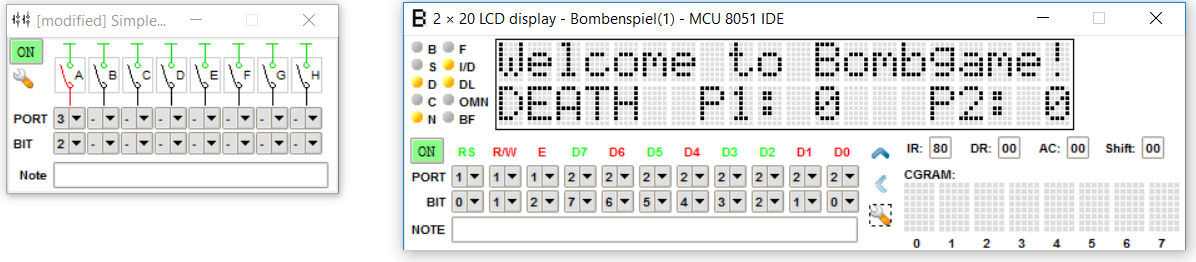
\includegraphics[scale=0.63]{img/Welcome}
	\caption{Willkommensnachricht}
\end{figure}

\begin{figure}[htbp]
	\centering
	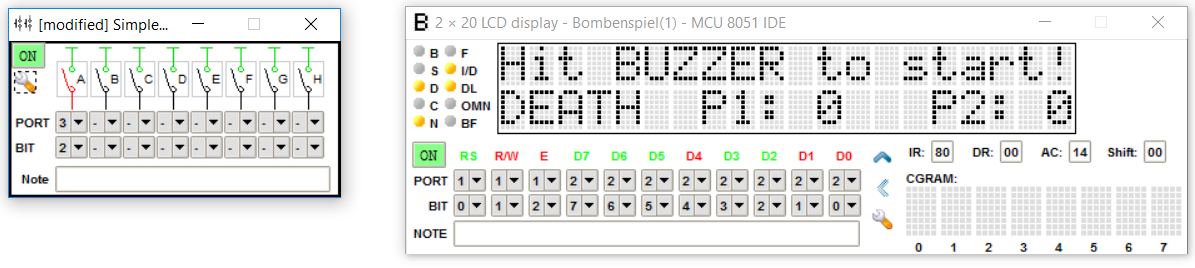
\includegraphics[scale=0.63]{img/StartGame}
	\caption{Startbildschirm}
\end{figure}

\begin{figure}[htbp]
	\centering
	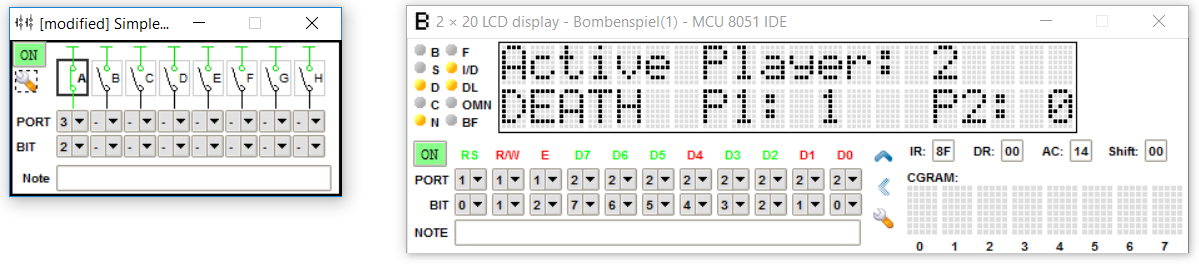
\includegraphics[scale=0.63]{img/Game}
	\caption{Spielablauf}
\end{figure}

\begin{figure}[htbp]
	\centering
	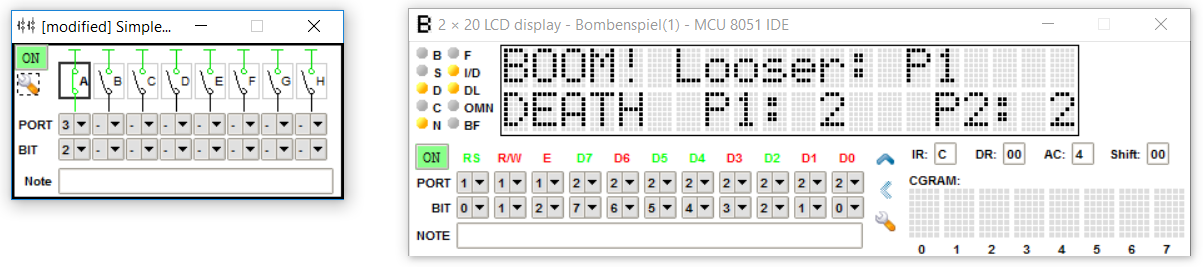
\includegraphics[scale=0.63]{img/Looser}
	\caption{Ende}
\end{figure}

\begin{appendix}

\bibliographystyle{unsrt}
\raggedright
\bibliography{references/bibliothek}

\noindent
\begin{minipage}{\textwidth}
	\listoffigures
\end{minipage}

\end{appendix}
	
\end{document}